\documentclass{article}

\usepackage{tikz}
\usetikzlibrary{calc}


\begin{document}\begin{figure}
   \tikzset{
      tick/.style = {black, very thick}
    }

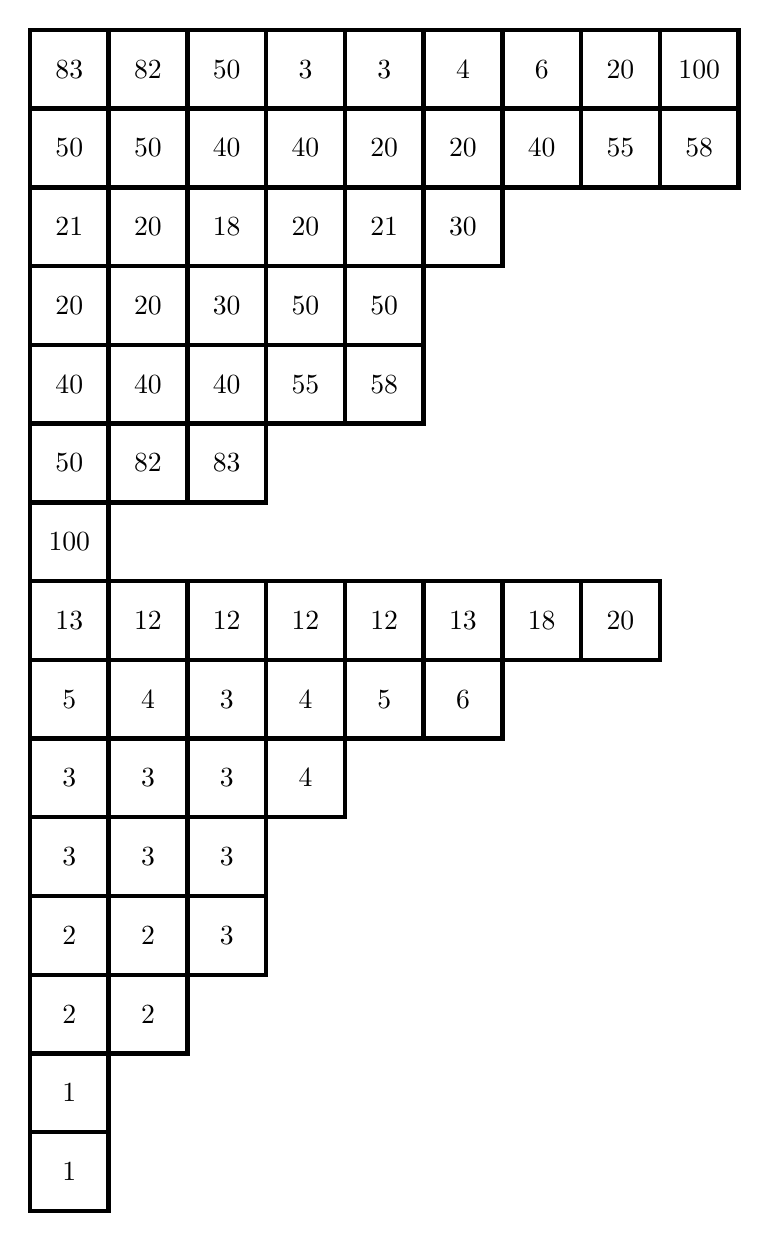
\begin{tikzpicture} % boxlength=1%ZEILE NR. 0 (von unten)

%ELEMENT IN SPALTE NR. 0 (von links)
\draw [ultra thick] (0,0) rectangle (1,1);
\node at ($(0.5,0.5)$) {$1$};




%ZEILE NR. 1 (von unten)

%ELEMENT IN SPALTE NR. 0 (von links)
\draw [ultra thick] (0,1) rectangle (1,2);
\node at ($(0.5,1.5)$) {$1$};




%ZEILE NR. 2 (von unten)

%ELEMENT IN SPALTE NR. 0 (von links)
\draw [ultra thick] (0,2) rectangle (1,3);
\node at ($(0.5,2.5)$) {$2$};

%ELEMENT IN SPALTE NR. 1 (von links)
\draw [ultra thick] (1,2) rectangle (2,3);
\node at ($(1.5,2.5)$) {$2$};




%ZEILE NR. 3 (von unten)

%ELEMENT IN SPALTE NR. 0 (von links)
\draw [ultra thick] (0,3) rectangle (1,4);
\node at ($(0.5,3.5)$) {$2$};

%ELEMENT IN SPALTE NR. 1 (von links)
\draw [ultra thick] (1,3) rectangle (2,4);
\node at ($(1.5,3.5)$) {$2$};

%ELEMENT IN SPALTE NR. 2 (von links)
\draw [ultra thick] (2,3) rectangle (3,4);
\node at ($(2.5,3.5)$) {$3$};




%ZEILE NR. 4 (von unten)

%ELEMENT IN SPALTE NR. 0 (von links)
\draw [ultra thick] (0,4) rectangle (1,5);
\node at ($(0.5,4.5)$) {$3$};

%ELEMENT IN SPALTE NR. 1 (von links)
\draw [ultra thick] (1,4) rectangle (2,5);
\node at ($(1.5,4.5)$) {$3$};

%ELEMENT IN SPALTE NR. 2 (von links)
\draw [ultra thick] (2,4) rectangle (3,5);
\node at ($(2.5,4.5)$) {$3$};




%ZEILE NR. 5 (von unten)

%ELEMENT IN SPALTE NR. 0 (von links)
\draw [ultra thick] (0,5) rectangle (1,6);
\node at ($(0.5,5.5)$) {$3$};

%ELEMENT IN SPALTE NR. 1 (von links)
\draw [ultra thick] (1,5) rectangle (2,6);
\node at ($(1.5,5.5)$) {$3$};

%ELEMENT IN SPALTE NR. 2 (von links)
\draw [ultra thick] (2,5) rectangle (3,6);
\node at ($(2.5,5.5)$) {$3$};

%ELEMENT IN SPALTE NR. 3 (von links)
\draw [ultra thick] (3,5) rectangle (4,6);
\node at ($(3.5,5.5)$) {$4$};




%ZEILE NR. 6 (von unten)

%ELEMENT IN SPALTE NR. 0 (von links)
\draw [ultra thick] (0,6) rectangle (1,7);
\node at ($(0.5,6.5)$) {$5$};

%ELEMENT IN SPALTE NR. 1 (von links)
\draw [ultra thick] (1,6) rectangle (2,7);
\node at ($(1.5,6.5)$) {$4$};

%ELEMENT IN SPALTE NR. 2 (von links)
\draw [ultra thick] (2,6) rectangle (3,7);
\node at ($(2.5,6.5)$) {$3$};

%ELEMENT IN SPALTE NR. 3 (von links)
\draw [ultra thick] (3,6) rectangle (4,7);
\node at ($(3.5,6.5)$) {$4$};

%ELEMENT IN SPALTE NR. 4 (von links)
\draw [ultra thick] (4,6) rectangle (5,7);
\node at ($(4.5,6.5)$) {$5$};

%ELEMENT IN SPALTE NR. 5 (von links)
\draw [ultra thick] (5,6) rectangle (6,7);
\node at ($(5.5,6.5)$) {$6$};




%ZEILE NR. 7 (von unten)

%ELEMENT IN SPALTE NR. 0 (von links)
\draw [ultra thick] (0,7) rectangle (1,8);
\node at ($(0.5,7.5)$) {$13$};

%ELEMENT IN SPALTE NR. 1 (von links)
\draw [ultra thick] (1,7) rectangle (2,8);
\node at ($(1.5,7.5)$) {$12$};

%ELEMENT IN SPALTE NR. 2 (von links)
\draw [ultra thick] (2,7) rectangle (3,8);
\node at ($(2.5,7.5)$) {$12$};

%ELEMENT IN SPALTE NR. 3 (von links)
\draw [ultra thick] (3,7) rectangle (4,8);
\node at ($(3.5,7.5)$) {$12$};

%ELEMENT IN SPALTE NR. 4 (von links)
\draw [ultra thick] (4,7) rectangle (5,8);
\node at ($(4.5,7.5)$) {$12$};

%ELEMENT IN SPALTE NR. 5 (von links)
\draw [ultra thick] (5,7) rectangle (6,8);
\node at ($(5.5,7.5)$) {$13$};

%ELEMENT IN SPALTE NR. 6 (von links)
\draw [ultra thick] (6,7) rectangle (7,8);
\node at ($(6.5,7.5)$) {$18$};

%ELEMENT IN SPALTE NR. 7 (von links)
\draw [ultra thick] (7,7) rectangle (8,8);
\node at ($(7.5,7.5)$) {$20$};




%ZEILE NR. 8 (von unten)

%ELEMENT IN SPALTE NR. 0 (von links)
\draw [ultra thick] (0,8) rectangle (1,9);
\node at ($(0.5,8.5)$) {$100$};




%ZEILE NR. 9 (von unten)

%ELEMENT IN SPALTE NR. 0 (von links)
\draw [ultra thick] (0,9) rectangle (1,10);
\node at ($(0.5,9.5)$) {$50$};

%ELEMENT IN SPALTE NR. 1 (von links)
\draw [ultra thick] (1,9) rectangle (2,10);
\node at ($(1.5,9.5)$) {$82$};

%ELEMENT IN SPALTE NR. 2 (von links)
\draw [ultra thick] (2,9) rectangle (3,10);
\node at ($(2.5,9.5)$) {$83$};




%ZEILE NR. 10 (von unten)

%ELEMENT IN SPALTE NR. 0 (von links)
\draw [ultra thick] (0,10) rectangle (1,11);
\node at ($(0.5,10.5)$) {$40$};

%ELEMENT IN SPALTE NR. 1 (von links)
\draw [ultra thick] (1,10) rectangle (2,11);
\node at ($(1.5,10.5)$) {$40$};

%ELEMENT IN SPALTE NR. 2 (von links)
\draw [ultra thick] (2,10) rectangle (3,11);
\node at ($(2.5,10.5)$) {$40$};

%ELEMENT IN SPALTE NR. 3 (von links)
\draw [ultra thick] (3,10) rectangle (4,11);
\node at ($(3.5,10.5)$) {$55$};

%ELEMENT IN SPALTE NR. 4 (von links)
\draw [ultra thick] (4,10) rectangle (5,11);
\node at ($(4.5,10.5)$) {$58$};




%ZEILE NR. 11 (von unten)

%ELEMENT IN SPALTE NR. 0 (von links)
\draw [ultra thick] (0,11) rectangle (1,12);
\node at ($(0.5,11.5)$) {$20$};

%ELEMENT IN SPALTE NR. 1 (von links)
\draw [ultra thick] (1,11) rectangle (2,12);
\node at ($(1.5,11.5)$) {$20$};

%ELEMENT IN SPALTE NR. 2 (von links)
\draw [ultra thick] (2,11) rectangle (3,12);
\node at ($(2.5,11.5)$) {$30$};

%ELEMENT IN SPALTE NR. 3 (von links)
\draw [ultra thick] (3,11) rectangle (4,12);
\node at ($(3.5,11.5)$) {$50$};

%ELEMENT IN SPALTE NR. 4 (von links)
\draw [ultra thick] (4,11) rectangle (5,12);
\node at ($(4.5,11.5)$) {$50$};




%ZEILE NR. 12 (von unten)

%ELEMENT IN SPALTE NR. 0 (von links)
\draw [ultra thick] (0,12) rectangle (1,13);
\node at ($(0.5,12.5)$) {$21$};

%ELEMENT IN SPALTE NR. 1 (von links)
\draw [ultra thick] (1,12) rectangle (2,13);
\node at ($(1.5,12.5)$) {$20$};

%ELEMENT IN SPALTE NR. 2 (von links)
\draw [ultra thick] (2,12) rectangle (3,13);
\node at ($(2.5,12.5)$) {$18$};

%ELEMENT IN SPALTE NR. 3 (von links)
\draw [ultra thick] (3,12) rectangle (4,13);
\node at ($(3.5,12.5)$) {$20$};

%ELEMENT IN SPALTE NR. 4 (von links)
\draw [ultra thick] (4,12) rectangle (5,13);
\node at ($(4.5,12.5)$) {$21$};

%ELEMENT IN SPALTE NR. 5 (von links)
\draw [ultra thick] (5,12) rectangle (6,13);
\node at ($(5.5,12.5)$) {$30$};




%ZEILE NR. 13 (von unten)

%ELEMENT IN SPALTE NR. 0 (von links)
\draw [ultra thick] (0,13) rectangle (1,14);
\node at ($(0.5,13.5)$) {$50$};

%ELEMENT IN SPALTE NR. 1 (von links)
\draw [ultra thick] (1,13) rectangle (2,14);
\node at ($(1.5,13.5)$) {$50$};

%ELEMENT IN SPALTE NR. 2 (von links)
\draw [ultra thick] (2,13) rectangle (3,14);
\node at ($(2.5,13.5)$) {$40$};

%ELEMENT IN SPALTE NR. 3 (von links)
\draw [ultra thick] (3,13) rectangle (4,14);
\node at ($(3.5,13.5)$) {$40$};

%ELEMENT IN SPALTE NR. 4 (von links)
\draw [ultra thick] (4,13) rectangle (5,14);
\node at ($(4.5,13.5)$) {$20$};

%ELEMENT IN SPALTE NR. 5 (von links)
\draw [ultra thick] (5,13) rectangle (6,14);
\node at ($(5.5,13.5)$) {$20$};

%ELEMENT IN SPALTE NR. 6 (von links)
\draw [ultra thick] (6,13) rectangle (7,14);
\node at ($(6.5,13.5)$) {$40$};

%ELEMENT IN SPALTE NR. 7 (von links)
\draw [ultra thick] (7,13) rectangle (8,14);
\node at ($(7.5,13.5)$) {$55$};

%ELEMENT IN SPALTE NR. 8 (von links)
\draw [ultra thick] (8,13) rectangle (9,14);
\node at ($(8.5,13.5)$) {$58$};




%ZEILE NR. 14 (von unten)

%ELEMENT IN SPALTE NR. 0 (von links)
\draw [ultra thick] (0,14) rectangle (1,15);
\node at ($(0.5,14.5)$) {$83$};

%ELEMENT IN SPALTE NR. 1 (von links)
\draw [ultra thick] (1,14) rectangle (2,15);
\node at ($(1.5,14.5)$) {$82$};

%ELEMENT IN SPALTE NR. 2 (von links)
\draw [ultra thick] (2,14) rectangle (3,15);
\node at ($(2.5,14.5)$) {$50$};

%ELEMENT IN SPALTE NR. 3 (von links)
\draw [ultra thick] (3,14) rectangle (4,15);
\node at ($(3.5,14.5)$) {$3$};

%ELEMENT IN SPALTE NR. 4 (von links)
\draw [ultra thick] (4,14) rectangle (5,15);
\node at ($(4.5,14.5)$) {$3$};

%ELEMENT IN SPALTE NR. 5 (von links)
\draw [ultra thick] (5,14) rectangle (6,15);
\node at ($(5.5,14.5)$) {$4$};

%ELEMENT IN SPALTE NR. 6 (von links)
\draw [ultra thick] (6,14) rectangle (7,15);
\node at ($(6.5,14.5)$) {$6$};

%ELEMENT IN SPALTE NR. 7 (von links)
\draw [ultra thick] (7,14) rectangle (8,15);
\node at ($(7.5,14.5)$) {$20$};

%ELEMENT IN SPALTE NR. 8 (von links)
\draw [ultra thick] (8,14) rectangle (9,15);
\node at ($(8.5,14.5)$) {$100$};






\end{tikzpicture}
\end{figure}
\end{document}